\documentclass{article}

\usepackage{graphicx}
\usepackage[utf8]{inputenc}
\usepackage[T1]{fontenc}
\usepackage[francais]{babel}
\usepackage{hyperref}
\usepackage{amsmath,amsfonts,amssymb}
\usepackage{Tkz-Tab}
\usepackage{wrapfig}
\usepackage{verbatim}
\usepackage{array}

\begin{document}

\title{Gestion de flux dans le réseau
	\smallbreak
	TD n\degre5
	\smallbreak
	Modélisation mathématique
	\smallbreak
	Q4}
\author{Sibylle Roux \and Juliette Arazo \and Nicolas Le Gallo \and Tanguy Thomas}

\maketitle

\newpage

\tableofcontents

\newpage

\section{Essaies randoms}

\subsection{Loi Hypergeometrique}

\subsection{Preuve mathématique}
\begin{align}
\intertext{Paramètres}
N=20 ; n=3 ; m = 2 : P = \frac{2}{20}
\\
P(X=0)=\frac{
\begin{pmatrix}
m \\ 0
\end{pmatrix}
\times 
\begin{pmatrix}
N - m \\ 3
\end{pmatrix}
}{
\begin{pmatrix}
N \\ n
\end{pmatrix}
} 
\end{align}
\begin{align}
P(X=0)=\frac{
\begin{pmatrix}
2 \\ 0
\end{pmatrix}
\times 
\begin{pmatrix}
18 \\ 3
\end{pmatrix}
}{
\begin{pmatrix}
20 \\ 3
\end{pmatrix}
}= \frac{\frac{18\times17\times16}{3\times2\times1}}{\frac{20\times19\times18}{3 \times 2}} = 0.7158
\end{align} 
\begin{align}
P(X=1)=\frac{
\begin{pmatrix}
2 \\ 1
\end{pmatrix}
\times 
\begin{pmatrix}
18 \\ 2
\end{pmatrix}
}{
\begin{pmatrix}
20 \\ 3
\end{pmatrix}
}= \frac{2 \times \frac{18\times17}{2}}{\frac{20\times19\times18}{3 \times 2}} = 0.2684
\end{align}
\begin{align}
P(X=2)=\frac{
\begin{pmatrix}
2 \\ 2
\end{pmatrix}
\times 
\begin{pmatrix}
18 \\ 1
\end{pmatrix}
}{
\begin{pmatrix}
20 \\ 3
\end{pmatrix}
}= \frac{1 \times 18}{\frac{20\times19\times18}{3 \times 2}} = 0.0158
\end{align}

\begin{verbatim}
clear
clc
function s=hypergeo(N,n,P)
    M=P*N;
    s=0;
    for i=0:n-1
        if rand()<P
            M=M-1;
            N=N-1;
            s=s+1;
            P=M/N;
        else
            N=N-1;
            P=M/N;
        end         
    end
endfunction
N=20; n=3; P=2/20;t=[]; nb=10000
for j=1:nb+1
    t(j)=hypergeo(N,n,P); //100 tirages de loi hypergeo
end
frequences=tabul(t)// on calcule les frequences obtenues
frequences(:,2)=frequences(:,2)/nb
disp(frequences)
\end{verbatim}

\paragraph{Resultats d'un essai}
\begin{center}
\begin{tabular}{cccc}
nombre de succès & 0 & 1 & 2 \\
\hline
resultats programme & 0.0172 & 0.2728 & 0.7101 \\
\hline
resultats mathématiques & 0.0158 & 0.2684 & 0.7158 \\
\hline
\end{tabular}
\end{center}
Les valeurs obtenues par le programme sont proches des valeurs mathématiques. On peut en conclure que le programme retranscrit bien une loi hypergéométrique.

\section{Etude mathématique de la loi tente}

\subsection{Densité}

\subsubsection{Fonction}

$$
f(x)=\left\{
	\begin{array}{ll}
		1-|x| & \mbox{si} -1<=x<=1\\
		0 & \mbox{sinon}
	\end{array}
\right.
$$

\subsubsection{Représentation graphique}
\begin{center}
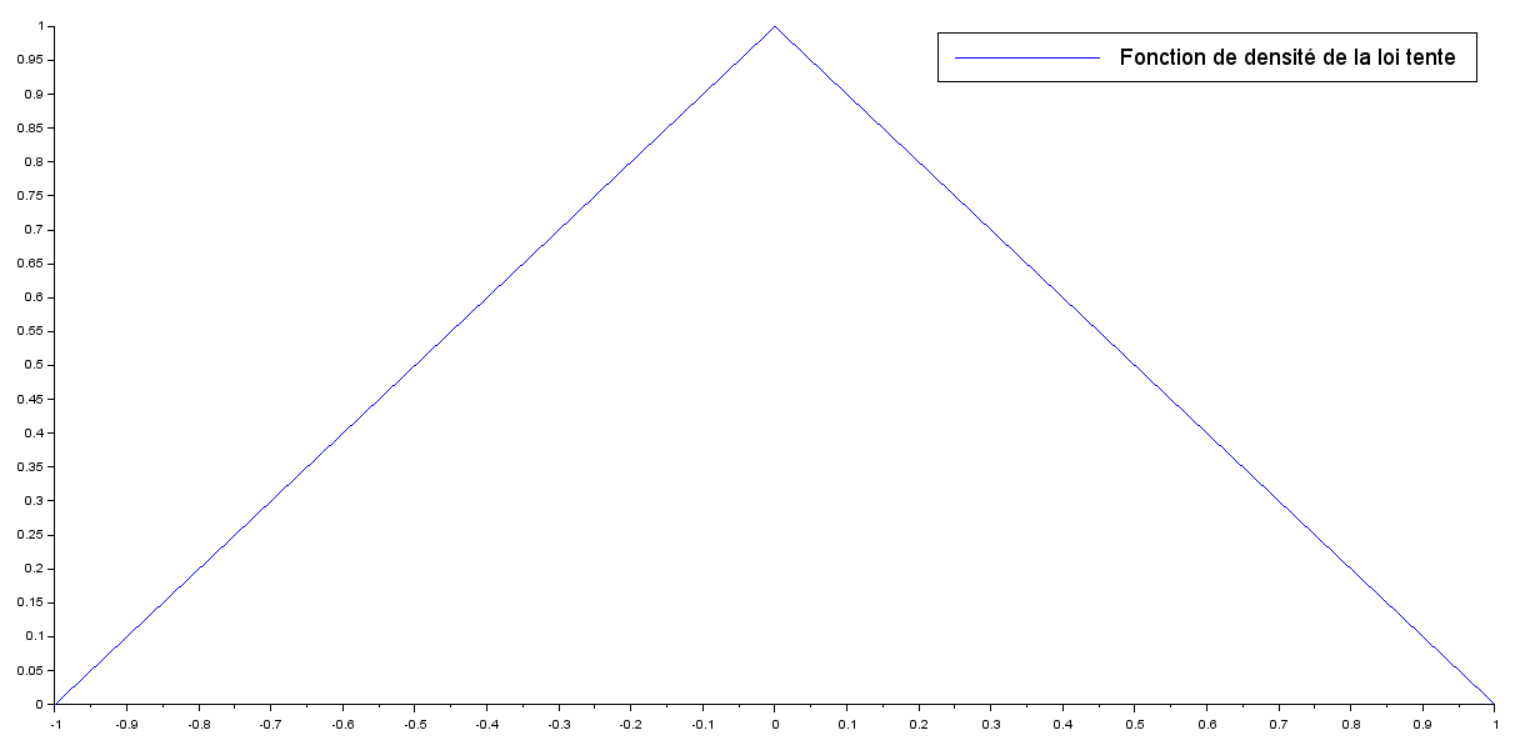
\includegraphics[width=425px]{img/tente.png}
\end{center}
\paragraph{}

\newpage

\subsection{Fonction de répartition}

\subsubsection{Fonction}

\begin{align}
f(x)=\left\{
	\begin{array}{llll}
		f(x)=0 &\mbox{pour } x<-1\\
		f(x)=1+x & \mbox{pour } -1<x<0 \\
		f(x)=1-x & \mbox{pour } 0<x<1 \\
		f(x)=0 & \mbox{pour } x>1 \\
	\end{array}
\right. 
\end{align}
\begin{align}
<=>
F(x)=\left\{
	\begin{array}{llll}
		\displaystyle \int_{- \infty }^{x} 0 \, \mathrm{d}x &\mbox{pour } x<-1\\
		\displaystyle \int_{- \infty }^{-1} 0 \, \mathrm{d}x+\displaystyle \int_{-1 }^{x} 1+x \, \mathrm{d}x &\mbox{pour } -1<x<0\\
		\displaystyle \int_{- \infty }^{-1} 0 \, \mathrm{d}x+\displaystyle \int_{-1 }^{0} 1+x \, \mathrm{d}x + \displaystyle \int_{0}^{x} 1-x \, \mathrm{d}x &\mbox{pour } 0<x<1\\
		\displaystyle \int_{- \infty }^{-1} 0 \, \mathrm{d}x+\displaystyle \int_{-1 }^{0} 1+x \, \mathrm{d}x + \displaystyle \int_{0}^{1} 1-x \, \mathrm{d}x+\displaystyle \int_{1}^{x} 0 \, \mathrm{d}x &\mbox{pour } x>1\\
	\end{array}
\right. 
\end{align}
\begin{align}
<=>
F(x)=\left\{
	\begin{array}{llll}
		0 &\mbox{pour } x<-1\\
		0 + \displaystyle \int_{-1 }^{x} 1+x \, \mathrm{d}x &\mbox{pour } -1<x<0\\
		0+\frac{1}{2}+\displaystyle \int_{0}^{x} 1-x \, \mathrm{d}x &\mbox{pour } 0<x<1\\
		0+\frac{1}{2}+\frac{1}{2}+\displaystyle \int_{1}^{x} 0 \, \mathrm{d}x &\mbox{pour } x>1\\
	\end{array}
\right. 
\end{align}
\begin{align}
<=>
F(x)=\left\{
	\begin{array}{llll}
		0 &\mbox{pour } x<-1\\
		\displaystyle \int_{-1 }^{x} 1+x \, \mathrm{d}x &\mbox{pour } -1<x<0\\
		\frac{1}{2}+\displaystyle \int_{0}^{x} 1-x \, \mathrm{d}x &\mbox{pour } 0<x<1\\
		1 &\mbox{pour } x>1\\
	\end{array}
\right. 
\end{align}
\begin{align}
<=>
F(x)=\left\{
	\begin{array}{llll}
		0 & \mbox{pour } x<-1\\
		\frac{1}{2} + x + \frac{x^2}{2} &\mbox{pour } -1<x<0\\
		\frac{1}{2} + x - \frac{x^2}{2} &\mbox{pour } 0<x<1\\
		1 & \mbox{pour } x>1\\
	\end{array}
\right.
\end{align}
\begin{align}
<=>
F(x)=\left\{
	\begin{array}{llll}
		0 & \mbox{pour } x<-1\\
		\frac{1}{2} \times (1 + 2x + x^2) &\mbox{pour } -1<x<0\\
		-\frac{1}{2} \times (-1 - 2x + x^2 +1 -1) &\mbox{pour } 0<x<1\\
		1 & \mbox{pour } x>1\\
	\end{array}
\right.
\end{align}
\begin{align}
<=>
F(x)=\left\{
	\begin{array}{llll}
		0 & \mbox{pour } x<-1\\
		\frac{(1+x)^2}{2} &\mbox{pour } -1<x<0\\
		\frac{2-(1-x)^2}{2} &\mbox{pour } 0<x<1\\
		1 & \mbox{pour } x>1\\
	\end{array}
\right.
\end{align}

\subsubsection{Représentation graphique}
\begin{center}
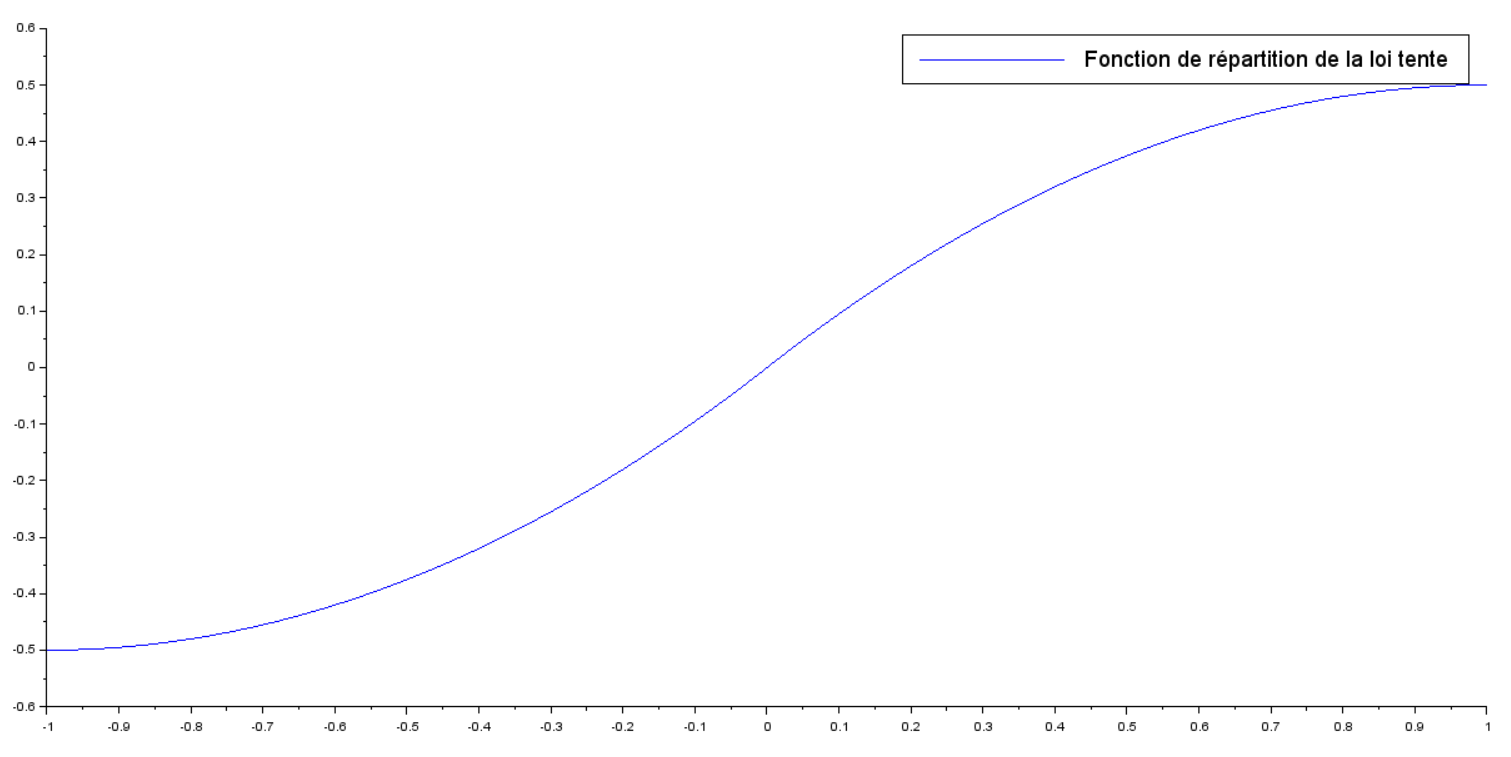
\includegraphics[width=425px]{img/tente_repartition.png}
\end{center}
\paragraph{}

\subsection{Inverse}

\subsubsection{Fonction}
\paragraph{} On va donc inverser les deux fonctions de répartitions de la loi tente \eqref{tente}

\begin{align}
\left\{
	\begin{array}{ll}
		y_1=\frac{(1+x)^2}{2} &\mbox{pour } -1<x<0\\
		y_2=\frac{2-(1-x)^2}{2} &\mbox{pour } 0<x<1\\
	\end{array}
\right.
%\label{tente}
\end{align}
\begin{align}
y_1 & =\frac{(1+x)^2}{2} & y_2 & = \frac{2-(1-x)^2}{2} \\
2y_1 & = (1+x)^2 & 2y_2 & = 2 - (1-x)^2 \\
\sqrt{2y_1} & = 1+x & 2-2y_2 & = (1-x)^2 \\
x & = \sqrt{2y_1} - 1 & x & = 1- \sqrt{ 2-2y_2}
\end{align}
\begin{align}
\intertext{Donc la fonction inverse est :}
F^{-1}(x)=\left\{
		\begin{array}{ll}
			\sqrt{2x}-1 & \mbox{pour} 0<x<\frac{1}{2} \\
			1-\sqrt{2-2x} & \mbox{pour} \frac{1}{2}<x<1
		\end{array}
\right.
\end{align}


\subsubsection{Représentation graphique}
\begin{center}
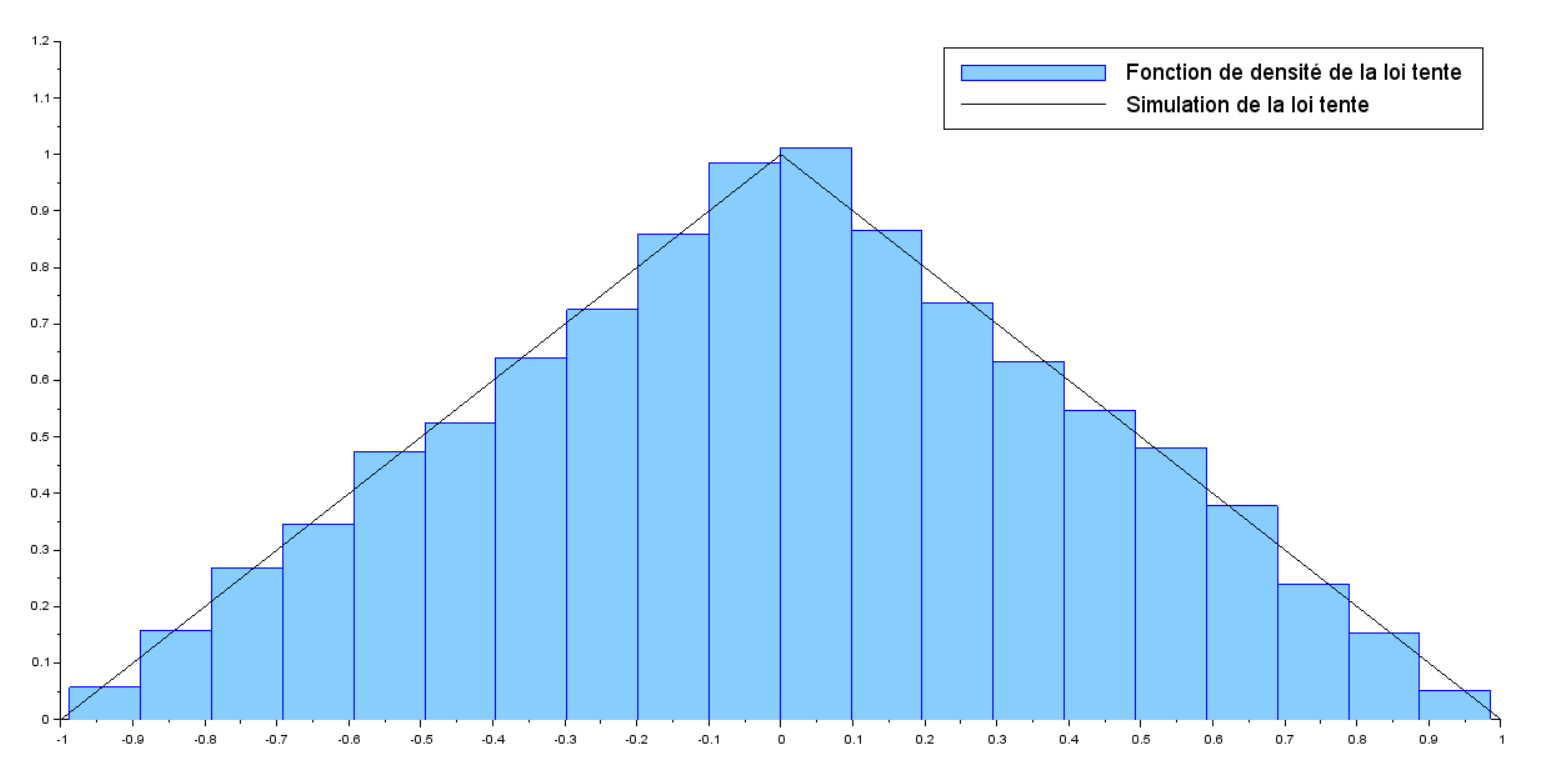
\includegraphics[width=425px]{img/tente_inversion.png}
\end{center}

\section{Inverse de la fonction de répartition de la loi exponentielle}

\subsection{Fonction}
\begin{align}
y & = 1 - e^{- \lambda t} \\
e^{- \lambda t} & =1-y \\
-\lambda t &= ln(1-y) \\
t &= - \frac{ln(1-y)}{\lambda}
\intertext{Donc la fonction inverse est : }
F^{-1}(t)&=- \frac{ln(1-y)}{\lambda}
\end{align}
\subsection{Représentation graphique}

\begin{center}
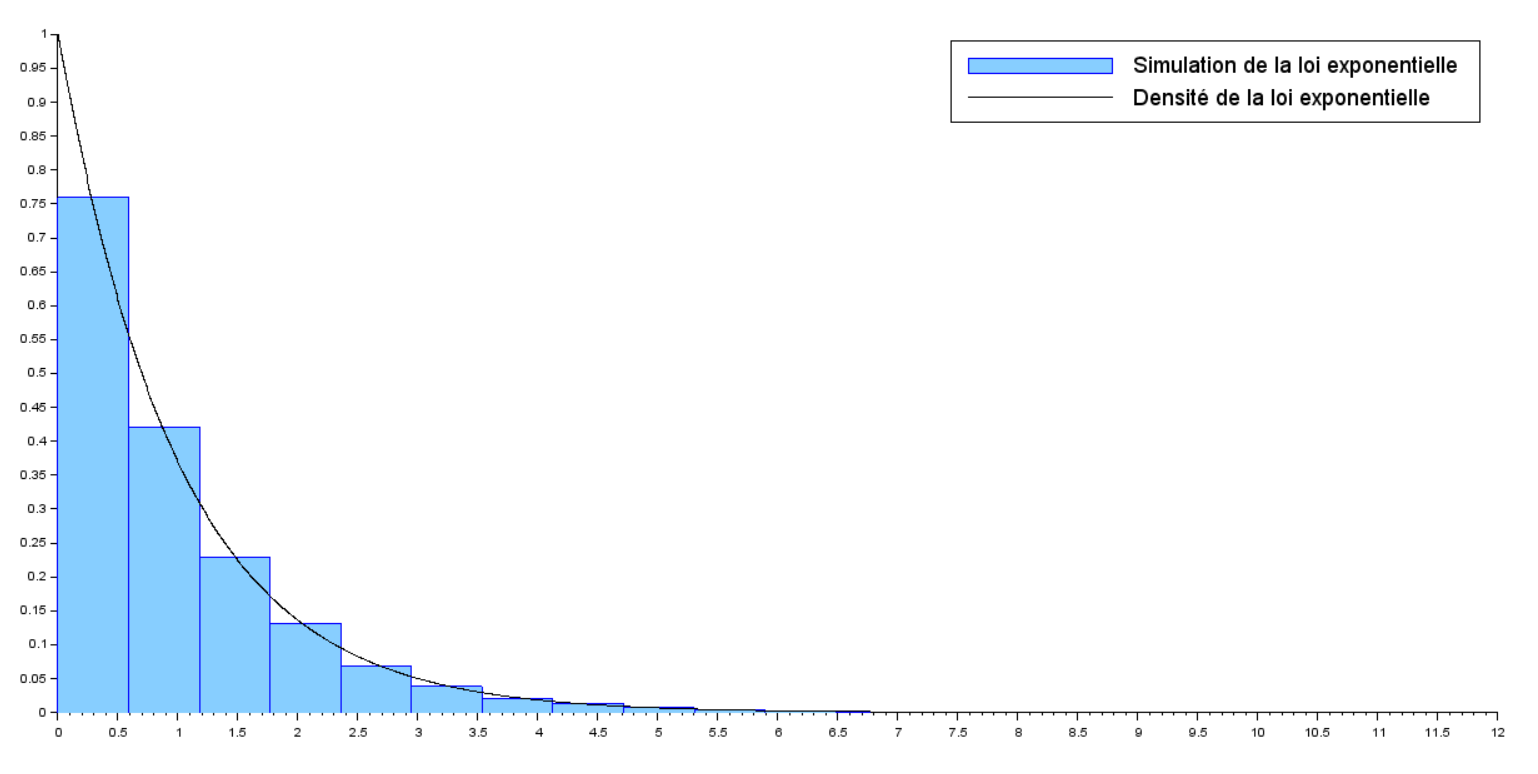
\includegraphics[width=425px]{img/inv_expo.png}
\end{center}
\paragraph{}

\section{Mesure de l'écart}

\subsection{Mesure de l'écart pour la loi tente}
\begin{center}
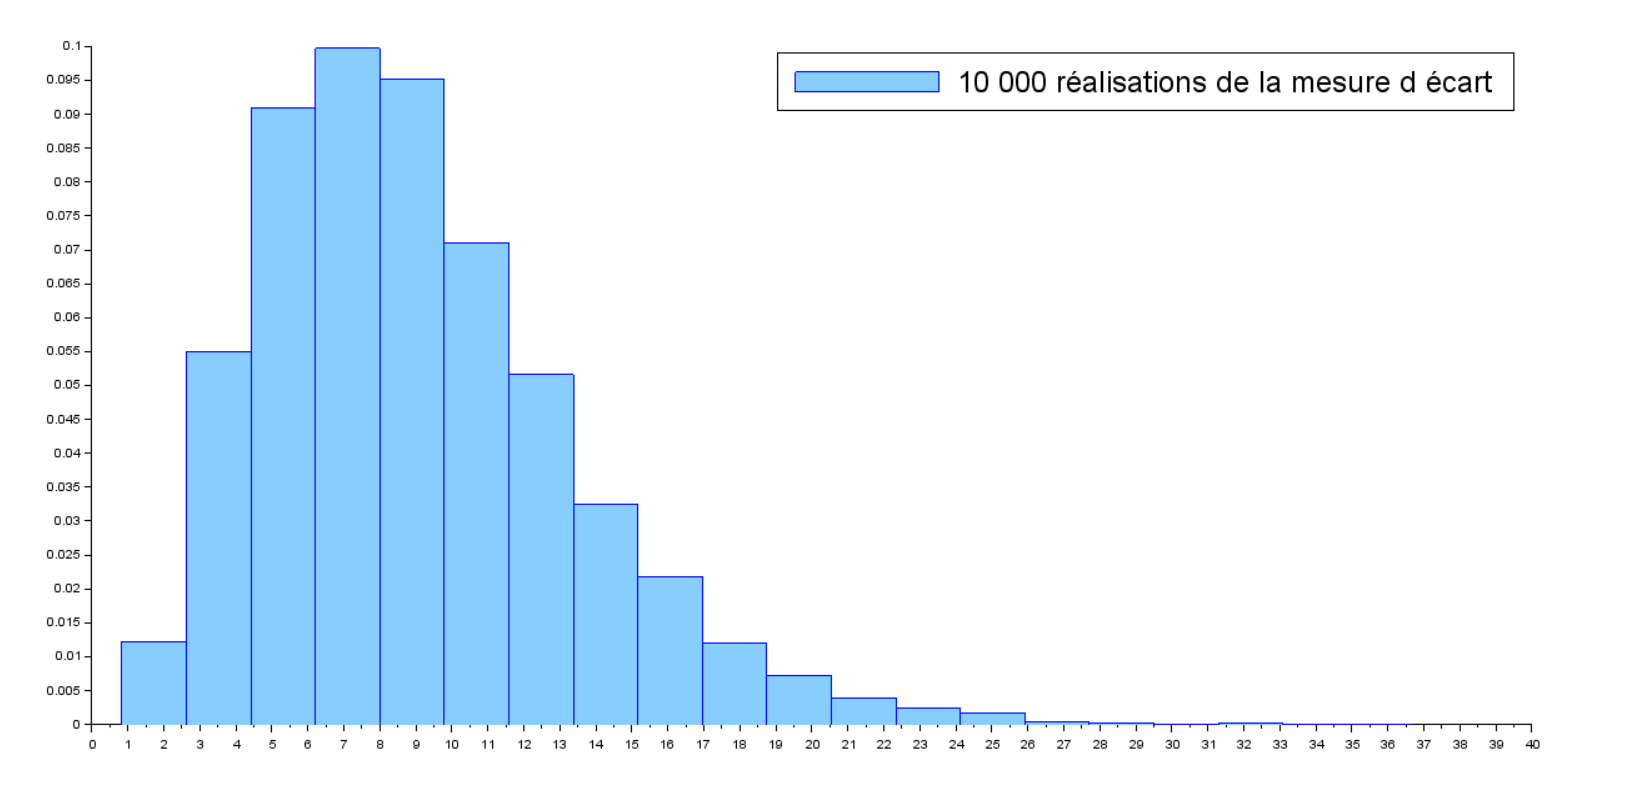
\includegraphics[width=425px]{img/ecart_tente.png}
\end{center}
\paragraph{}
Ce graphique représente l’histogramme de l’écart entre les valeurs théoriques et empiriques de 10 000 réalisations, pour la loi tente.  On peut voir que la grande majorité des écarts se situe entre 5 et 10. Cependant, on constate qu’à cause de  la fluctuation d’échantillonnage, certains écarts sont très importants.  Il est donc essentiel de se donner une marge d’erreur, afin de pouvoir affirmer avec une relative certitude si un échantillon donné suit une loi tente. 
Dans notre cas, on sait que 95\% des écarts sont inférieurs à  16.65: on pourra donc conclure qu’un échantillon suit une loi tente si il ne dépasse pas le seuil de 16.65.


\subsection{Mesure de l'écart pour la loi exponentielle}
\begin{center}
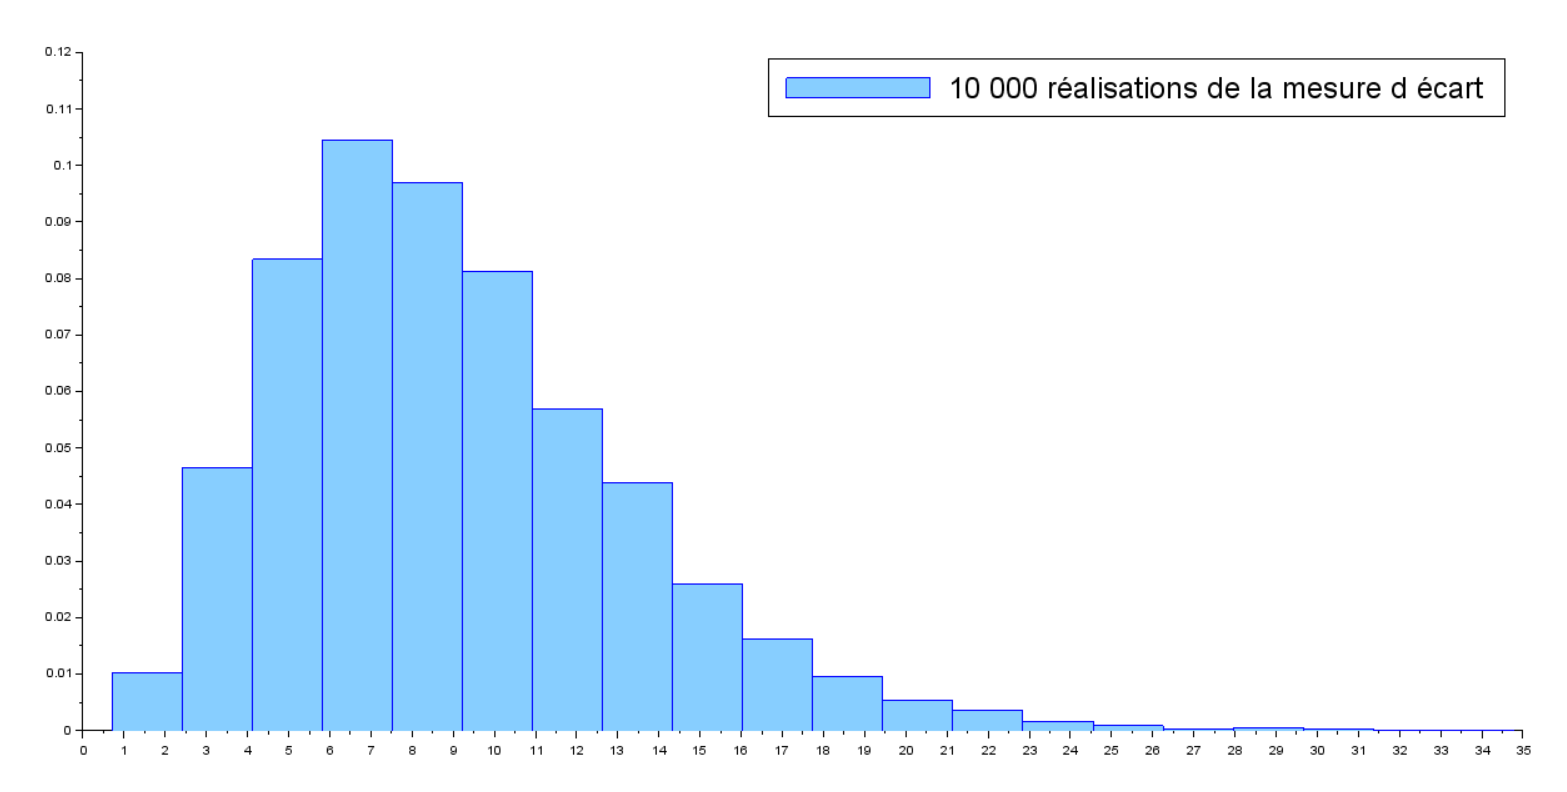
\includegraphics[width=425px]{img/ecart_expo.png}
\end{center}
\paragraph{}
Comme pour le graphique précédent, celui-ci représente l’histogramme des écarts sur 10 000 réalisations, cette fois-ci pour la loi exponentielle de paramètre lambda=1. Ici, la plupart des écarts se situent entre 4 et 11. Néanmoins on observe toujours des valeurs très distante de la moyenne, on va donc aussi utiliser une marge d’erreur à 95\%: dans ce cas, 95\% des écarts sont inférieurs à 17,1, qui sera donc le seuil à ne pas dépasser pour qu’un échantillon suive une loi exponentielle.

\subsection{Mesure de l'écart entre les données et la loi exponentielle}
\paragraph{}
Lorsqu’on calcule l’écart entre les mesures réalisées dans le dernier rapport ( temps inter-arrivés), qui semblaient suivre une loi exponentielle,  et une loi exponentielle, toutes deux de même paramètre $ \lambda = 1/moyenne(t_ia)$ , l’écart mesuré est de 14 . Or, 14 est inférieur au seuil 17, on peut donc estimer de façon assez certaine que les temps inter-arrivées suivent une loi exponentielle.

\paragraph{}
Nous allons faire de même pour les temps de service des trois serveurs, qui semblent aussi suivre des loi exponentielles de paramètre $\lambda = 1/moyenne(temps de service)$. On obtient les écarts suivants :
\begin{center}
\begin{tabular}{cccc}
Serveur & 1 & 2 & 3 \\
\hline
Ecarts & 8.1 & 4.02 & 7.07 \\
\hline
\end{tabular}
\end{center}
\paragraph{}
Ainsi, on constate que les trois serveurs ont des temps de service qui suivent une loi exponentielle de paramètre $\lambda= 1/moyenne(temps de service)$.
\section{Conclusion}
\paragraph{}

\newpage
\appendix

\section{Etude mathématique de la loi tente}
\subsection{Représentation graphique de la densité}
\begin{verbatim}
t = linspace(-1, 1, 301);
T = t;
i1 = (t>=-1) & (t<=1);
i2 = t>1 & t<-1;
T(i1)=1-abs(T(i1));
T(i2)=0
plot2d(t,T,style=2)
legend("Fonction de densité de la loi tente")
\end{verbatim}

\subsection{Représentation graphique de la fonction de répartition}
\begin{verbatim}
t = linspace(-1, 1, 301);
R=t;
i1 = t<-1;
i2 = (t>=-1) & (t<=0);
i3 = (t>0) & (t<=1);
i4 = t>1;
R(i1) = 0;
R(i2) = 0.5 + R(i2)+((R(i2)^2)/2)
R(i3) = 0.5 + R(i3)-((R(i3)^2)/2)
R(i4) = 1;
plot2d(t,R,style=2)
legend("Fonction de répartition de la loi tente")
\end{verbatim}

\subsection{Représentation graphique de la fonction inverse}
\begin{verbatim}
function t = tente(n)
    u = rand(n, 1);
    t = u
    i1 = u < 1/2
    i2 = u >= 1/2
    t(i1) = sqrt(2*t(i1))-1;
    t(i2) = 1-sqrt(2-2*t(i2));
endfunction
histplot(20,tente(10000))

// Fonction de densité 

t = linspace(-1, 1, 301);
T = t;
i1 = (t>=-1) & (t<=1);
i2 = t>1 & t<-1;
T(i1)=1-abs(T(i1));
T(i2)=0
plot2d(t,T,style=1)

legend("Fonction de densité de la loi tente","Simulation de la loi tente")
\end{verbatim}

\section{Inverse de la fonction de répartition}

\subsection{Représentation graphique de la fonction inverse}
\begin{verbatim}
function t = expo(l,n)
    u = rand(n, 1);
    t = u
    t = -log(1-t)/l 
endfunction
histplot(20,expo(1,100000))

// Fonction de densité de la loi exponentielle

a=0:0.01:12;
lambda=1;
b=lambda*exp(-lambda*a);
plot2d2(a,b,style=1)

legend("Simulation de la loi exponentielle","Densité de la loi exponentielle")
\end{verbatim}

\section{Mesure de l'écart}

\subsection{Mesure de l'écart pour la loi tente}
\begin{verbatim}
function q = quantile(p)
    if p < 0.5 then
        q = sqrt(2*p)-1;
    else
        q = 1-sqrt(2-2*p)
    end
endfunction

function t = tente(n)
    u = rand(n, 1);
    t = u
    i1 = u < 1/2
    i2 = u >= 1/2
    t(i1) = sqrt(2*t(i1))-1;
    t(i2) = 1-sqrt(2-2*t(i2));
endfunction

n = 10;
C = zeros(1, n + 1)
C(1) = -1; C(n+1) = 1; 
for i = 1:(n-1)
    C(i+1) = quantile(i/n);
end
format(6)

Ei = 3000 / n // effectif espéré dans chaque classe

N = 10000
d = zeros(1, N);
for i = 1:N
    Oi = histc(C, tente(3000), normalization = \%f);
    // calcul de la différence et stockage dans le tableau d
    d(i) = sum((Oi - Ei) .^2 ./ Ei); 
end

histplot(20,d)
legend("10 000 réalisations de la mesure d écart")

seuil=perctl(d,95)
\end{verbatim}

\subsection{Mesure de l'écart pour la loi exponentielle}
\begin{verbatim}
function q = quantile(l,p)
    q = -log(1-p)/l
endfunction

function t = expo(l,n)
    u = rand(n, 1);
    t = u
    t = -log(1-t)/l
endfunction

lambda=1;

n = 10;
C = zeros(1, n + 1)
C(1) = 0; C(n+1) = 1000000000000; 
for i = 1:(n-1)
    C(i+1) = quantile(lambda,i/n);
end
format(6)

Ei = 3000 / n // effectif espéré dans chaque classe

N = 10000
d = zeros(1, N);
for i = 1:N
    Oi = histc(C, expo(lambda,3000), normalization = \%f);
    d(i) = sum((Oi - Ei) .^2 ./ Ei);
end

histplot(20,d)
legend("10 000 réalisations de la mesure d écart")

seuil=perctl(d,95)
\end{verbatim}

\subsection{Mesure de l'écart entre les données et la loi exponentielle}
\begin{verbatim}
// Extraction des temps inter-arrivées
t_ia = data(2:$, 2) - data(1:1237, 2);

function q = quantile(l,p)
    q = -log(1-p)/l
endfunction

lambda=1/mean(t_ia);

n = 10;
C = zeros(1, n + 1)
C(1) = 0; C(n+1) = 100; 
for i = 1:(n-1)
    C(i+1) = quantile(lambda,i/n);
end
format(6)

Ei = 1237 / n // effectif espéré dans chaque classe

Oi = histc(C, t_ia, normalization = \%f);
d = sum((Oi - Ei) .^2 ./ Ei);
\end{verbatim}

%----------------------------------

 \subsection{Mesure de l'écart pour les temps de service du serveur 1}
\begin{verbatim}
// Extraction des temps de service
index_bool = ( data(:, 3) == 1 )
tabS1 = data(index_bool, :)
t_s1 = tabS1(1:$,4);

function q = quantile(l,p)
    q = -log(1-p)/l
endfunction

lambda=1/mean(t_s1);

n = 10;
C = zeros(1, n + 1)
C(1) = 0; C(n+1) = 10000; 
for i = 1:(n-1)
    C(i+1) = quantile(lambda,i/n);
end
format(6)

Ei = 412 / n // effectif espéré dans chaque classe

Oi = histc(C, t_s1, normalization = \%f);
d = sum((Oi - Ei) .^2 ./ Ei);
\end{verbatim}

 \subsection{Mesure de l'écart pour les temps de service du serveur 2}
\begin{verbatim}
// Extraction des temps de service
index_bool = ( data(:, 3) == 2 )
tabS1 = data(index_bool, :)
t_s1 = tabS1(1:$,4);

function q = quantile(l,p)
    q = -log(1-p)/l
endfunction

lambda=1/mean(t_s1);

n = 10;
C = zeros(1, n + 1)
C(1) = 0; C(n+1) = 10000; 
for i = 1:(n-1)
    C(i+1) = quantile(lambda,i/n);
end
format(6)

Ei = 413 / n // effectif espéré dans chaque classe

Oi = histc(C, t_s1, normalization = \%f);
d = sum((Oi - Ei) .^2 ./ Ei);
\end{verbatim}

 \subsection{Mesure de l'écart pour les temps de service du serveur 3}
\begin{verbatim}
// Extraction des temps de service
index_bool = ( data(:, 3) == 3 )
tabS1 = data(index_bool, :)
t_s1 = tabS1(1:$,4);

function q = quantile(l,p)
    q = -log(1-p)/l
endfunction

lambda=1/mean(t_s1);

n = 10;
C = zeros(1, n + 1)
C(1) = 0; C(n+1) = 10000; 
for i = 1:(n-1)
    C(i+1) = quantile(lambda,i/n);
end
format(6)

Ei = 413 / n // effectif espéré dans chaque classe

Oi = histc(C, t_s1, normalization = \%f);
d = sum((Oi - Ei) .^2 ./ Ei);
\end{verbatim}
\end{document}